\documentclass{article}

\usepackage{swiftnav}


\usepackage{draftwatermark, array}
\SetWatermarkLightness{0.9}
\SetWatermarkText{Preliminary}
\SetWatermarkScale{1}
% Suppress numbers from section headings (but preserve PDF TOC).
\makeatletter
\renewcommand\@seccntformat[1]{}
\makeatother
\newcolumntype{$}{>{\global\let\currentrowstyle\relax}}
\newcolumntype{^}{>{\currentrowstyle}}
\newcommand{\rowstyle}[1]{\gdef\currentrowstyle{#1}%
  #1\ignorespaces
}
\newenvironment{mpar}{\par\noindent\minipage{\linewidth}}{\endminipage\par}
%\setlength{\skip\mpfootins}{2cm}
\renewcommand{\thempfootnote}{(\arabic{mpfootnote})}


% ---------------------------------------------------------------------------
\usepackage[section]{placeins}
\version{0.1}
\title{Piksi for UAV Aerial surveying}
\mysubtitle{RTK direct georeferencing with Swift Navigation's Piksi GPS receiver}
\author{Dennis Zollo, Rai Gohalwar}
\date{\today}

\ignorespaces

\begin{document}
\maketitle

\thispagestyle{firstpage}

\section{Abstract}
\label{sec:abstract}
This whitepaper presents using Piksi, a Carrier Phase differential GPS sensor, to georeference aerial images from micro aerial vehicles (MAVS) for surveying use cases.
It presents both the sensor integration, data collection methods, and real world surveying results as processed by the PIX4D photogrammetry software.  Lastly, the value proposition of using RTK GPS for aerial surveying is evaluated.
\tableofcontents
\newpage
\section{Overview}
\label{sec:Overview}
Due to the impressive capability, low-cost, and increasing popularity of micro aerial vehicles, there is much interest and excitement about the potential applications of the aircraft in the future. One promising application for is aerial surveying for industries such as precision agriculture, mining, and forestry.

In a typical aerial surveying use-case, a fixed wing or multi-rotor aircraft is outfitted with a high-quality camera.  The vehicle overflies the area of interest and captures a series of images which are processed in software to produce Digital Elevation Models (DEM's), Orthomosaics, and 3D point clouds.  These models and deliverables, in turn, can be used for photogrammetry applications, volumetric measurements, or crop health measurements which can provide business value for the target use case.

Commercial software tools for photogrammetry have the ability to stitch together aerial images through visual features with techniques such as Bundle adjustment [TODO: Citations].  These software packages often require rough location and orientation of the lense when the photo was taken. To that end, most low-cost MAV control systems used for photogrammetry have the ability to geotag photos as required by the processing software. These vehicles often employ Autonomous or Single Point GPS combined with MEMS sensors to measure this information.  The typical sensor technology, combined with uncertainty in timing of the camera's shutter, limits the precision and accuracy of geotagging information and requires post-processing software to rely heavily on image processing techniques. Additionally, large amounts of sidelap and overlap between images is often required to allow post-processing software to utilize imagery information given the inaccuracy of the georeferencing information.  Lastly, survey sites lacking in visual detail (such as agricultural land) or where overlap is minimal (such as corridor mapping), often yield poor results with traditional techniques and sensors.

It has been demonstrated that Carrier Phase Differential GPS (Also called Real Time Kinematic (RTK)), can improve the location accuracy of geo-referencing [Cite XBEE or other stuff here].  This paper will demonstrate methods to use Swift Navigation's Piksi GPS Receiver to this end and evaluate any performance improvements.

\section{Equipment and Setup}
\label{sec:equipment}in
here we describe the equipment
\begin{table}[]
\centering
\label{my-label}
\begin{tabular}{|l|c|}
\hline
\multicolumn{2}{|c|}{Vehicle Specifications} \\ \hline
Frame Type            & Quad-Rotor           \\ \hline
Frame                 & Tarot FY650          \\ \hline
Flight Controller     & 3DR Pixhawk          \\ \hline
Motors x 4            & T-Motor MN4006       \\ \hline
Motor Controllers x 4 & X-Rotor 40A OPTO     \\ \hline
Propellers x 4        & Tarot 1555 CF        \\ \hline
Batteries x 2         & Multistar 6S 5200mAh \\ \hline
Weight                & 2942 g               \\ \hline
\end{tabular}
\end{table}
\begin{table}[]
\centering
\label{my-label}
\begin{tabular}{|l|c|}
\hline
\multicolumn{2}{|c|}{Camera Specifications}                                                \\ \hline
Camera                                                                & Sony Nex-5T        \\ \hline
Lens                                                                  & Sony SEL-20F28     \\ \hline
\begin{tabular}[c]{@{}l@{}}Weight\\ (with vehicle mount)\end{tabular} & 424 g              \\ \hline
Sensor                                                                & 16 MP: 4912 x 3264 \\ \hline
\end{tabular}
\end{table}
\begin{table}[]
\centering
\label{my-label}
\begin{tabular}{|l|c|}
\hline
\multicolumn{2}{|c|}{GPS Specifications} \\ \hline
Primary GPS         & Piksi v2.3.1       \\ \hline
Secondary GPS       & U-Blox NEO 7N      \\ \hline
Primary Antenna     & Tellysman TW2412   \\ \hline
Secondary Antenna   & Taoglas gp.1575    \\ \hline
\end{tabular}
\end{table}
Camera, focal length, quadcopter
Radios
\section{Method}
\label{sec:method}
Site selection
GCP surveying (skylark)
Mission Planning (mission planner)
Camera setup (exposure, etc)
\section{Post-Processing Techniques}
\begin{figure}
\begin{center}
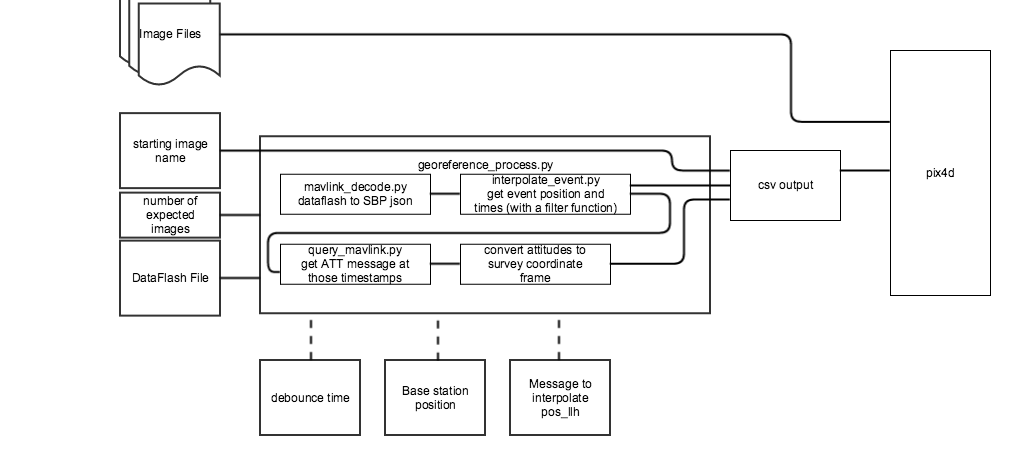
\includegraphics[width=7in]{images/uav_survey_processing_architecture.png}
\end{center}
\end{figure}

\begin{tabular}{l ^ l ^ l ^ l ^ l} \hline
\rowstyle{\bfseries}
Configuration & Description & Pix4D Calibration Method & GPS Sensor & Ground Control \\ \hline
\rowstyle{}
A & Piksi RTK Std & Standard & Piksi RTK (Fixed) & None  \\ \hline
B& Piksi RTK Std & Standard & Piksi RTK (Fixed) & 7 GCPS  \\ \hline
C & Piksi RTK Acc & Accurate & Piksi RTK (Fixed) & None  \\ \hline
D & Piksi RTK Acc & Accurate & Piksi RTK (Fixed) & 7 GCPS  \\ \hline
E & Ublox STD & Standard & UBLOX & None  \\ \hline
F & Ublox STD & Standard & UBLOX & 7 GCPS  \\ \hline
G & Ublox Acc & Accurate & UBLOX & None  \\ \hline
H & Ublox Acc & Accurate & UBLOX & 7 GCPS  \\ \hline
\end{tabular}
\section{Results: Accuracy}
talk about accuracy of each method
\section{Results: Overlap/Sidelap}
Show that overlapp can be reduced with accurate geotag
\thispagestyle{lastpage}
\end{document}
